% !TEX root = ../../buch.tex
% einleitung.tex -- Beispiel-File für die Einleitung
%
% (c) 2020 Prof Dr Andreas Müller, Hochschule Rapperswil
%
\section{Einleitung \label{burgers:section:einleitung}}
\rhead{Einleitung}

	Die Gleichung von Burgers,
	\begin{equation}
		  \frac {\partial u}{\partial t}+u{\frac {\partial u}{\partial x}}=\nu {\frac {\partial ^{2}u}{\partial x^{2}}},
		  \label{burgers:eq_burgers}
	\end{equation}
	ist eine nichtlineare partielle Differentialgleichung.
	Das Definitionsgebiet
	\begin{equation}
		\Omega = \left \{ (x,t) \in  \mathbb{R} \,\, \times \,\,  \mathbb{R}^t \right \}
	\end{equation}
	besteht aus der Dimension $x$ und der Zeit $t$.
	Die Gleichung von Burgers $u(t,x)$ ist in $\Omega$ definiert, wobei die Anfangswerte $u(0,x)$ bekannt sein müssen.
	In diesem Paper wird die reibungsfreie Burgersgleichung,
	\begin{equation}
		\frac {\partial u}{\partial t}+u{\frac {\partial u}{\partial x}}=0,
		\label{burgers:eq_invisid_burgers}
	\end{equation}
	betrachtet, wobei der Diffusionsterm $\nu$ auf 0 gesetzt wird.


	Das Aussergewöhnliche an der Gleichung ist die Nichtlinearität, diese erschwert die numerische L\"osung erheblich.

	Als Beispiel, kann f\"ur die Randbedingung bei $u(0,x)$ eine Normalverteilung verwendet werden.
	Die gel\"oste Gleichung kann in \autoref{burgers:fig:b1} betrachtet werden.

	    \begin{figure}
		\centering
		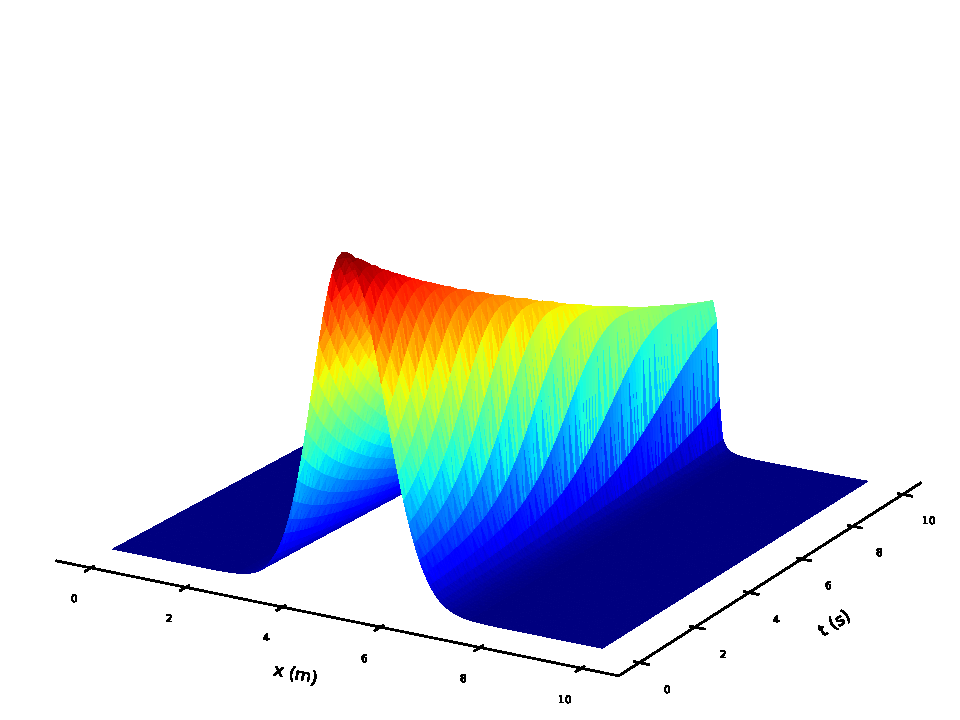
\includegraphics[width=.49\textwidth]{papers/burgers/BurgersEquation/images/Implicit_front.pdf}
		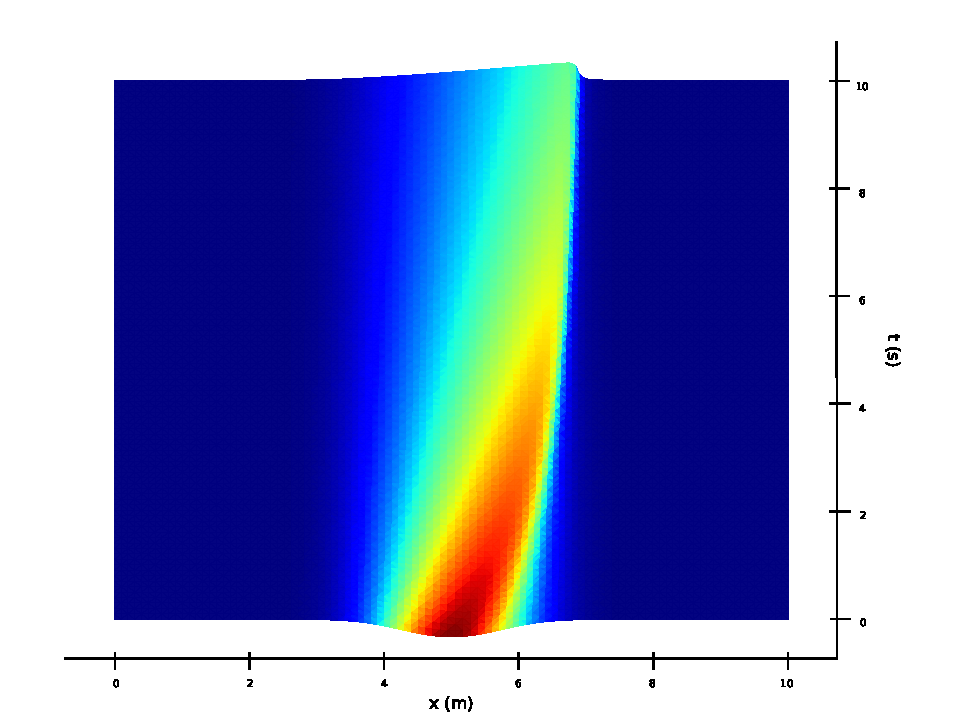
\includegraphics[width=.49\textwidth]{papers/burgers/BurgersEquation/images/Implicit_top.pdf}
		\caption{Gel\"oste Burgersgleichung}
		\label{burgers:fig:b1}
		\end{figure}


	\subsection{Beziehung zu den Navier Stokes Gleichungen}
		Die Gleichung wird häufig für die Modelierung von Fluiden verwendet.
		Namentlich wird sie gebraucht um die Navier Stokes Gleichungen zu vereinfachen.
		Die Navier Stokes Gleichungen beschreiben die Str\"omung von Fluiden.
		Die Gleichung von Burgers kann aus der Navier Stokes Gleichung f\"ur newtonsche inkompressible Fluide

		\begin{equation}
			\rho \left(\frac{\partial u}{\partial t} + u \, \nabla u \right) = -\nabla p + \mu \nabla^2 u + F
			\label{burgers:eq_navier}
		\end{equation}
		hergeleitet werden \cite{burgers:navier}.
		Wenn der Druck $p$ und die externe Kraft $F$ vernachl\"asigt wird, ergibt sich
		\begin{equation}
			\rho \left(\frac{\partial u}{\partial t} + u \, \nabla u \right) = \mu \nabla^2 u
			 \label{burgers:eq_navier2}
		\end{equation}
		Die Dichte $\rho$ kann mit der Geschwindigkeit des Vektorfeldes $\mu$ zur Konstante $\nu = \frac{\mu}{\rho}$
		\begin{equation}
			 \frac{\partial u}{\partial t} + u \,\nabla u = \nu \nabla^2 u
			 \label{burgers:eq_navier3}
		\end{equation}
		umgeschrieben werden.
		Wie bereits erw\"ahnt wird die reibungsfreie Gleichung betrachten ($\nu = 0$), weiter werden die kommenden Betrachtungen im eindimensionalen Raum durchgef\"uhrt.
		Somit kann der Ableitungsoperator $\nabla$ als die Ableitung im Raum $x$ umgeschrieben werden.
		Mit diesen Vereinfachungen der Navier Stokes Gleichung f\"ur newtonsche inkompressible Fluide ist man bei der urspr\"unglichen Gleichung \eqref{burgers:eq_invisid_burgers} angelangt.

	%\subsection{Numerische Wetter Vorhersage}
	%	Lewis Fry Richardson (1881 - 1953) war ein Britischer Mathematiker/Physiker.
